\chapter{Kuznyechik}

Kuznyechik là một thuật toán mã hóa khối, đối xứng như AES. Kuznyechik
tiếng Nga là \foreignlanguage{russian}{Кузнечик}, có nghĩa là châu chấu.
Tuy nhiên trong văn bản quốc tế thì chúng ta giữ nguyên tên gọi
là hệ mã Kuznyechik.

Mã khối Kuznyechik biến đổi trên khối 128 bit, độ dài khóa là
256 bit, biến đổi trên 9 vòng. Kuznyechik sử dụng mô hình SPN
tương tự như AES, trở thành chuẩn mã hóa của Nga và được định 
nghĩa trong GOST R 34.12-2015.

Một điểm đặc biệt là quá trình biến đổi qua các vòng sử dụng mạng
SPN, tuy nhiên thuật toán sinh khóa con cho các vòng sử dụng
mô hình Feistel.

Phần này tham khảo chính từ \cite{Losi}.

\section{Mã hóa}

Gọi $k_i$ là khóa con của vòng thứ $i$, $i = 0, 1, \ldots, 9$. 
Ta có các động tác biến đổi sau:

\textbf{1.} Hàm $X: \FF_2^{128} \to \FF_2^{128}$ biến đổi
trên block 128 bit.

Ta chia block đầu vào thành 16 cụm 8 bit, ký hiệu
\[a = a_0 \Vert a_1 \Vert \ldots \Vert a_{14} \Vert a_{15}\]
với ký tự $\Vert$ chỉ việc nối các chuỗi bit (concatenate).
Tương tự $k_i$ cũng được chia thành 16 cụm 8 bit. Khi đó, 
\begin{equation}
    \label{kuz:1}
    X(k_i, a) = k_{i, 0} \oplus a_0 \Vert 
    k_{i, 1} \oplus a_1 \Vert \ldots \Vert k_{i, 14} \oplus a_{14}
    \Vert k_{i, 15} \oplus a_{15}
\end{equation}

Nói cách khác, chúng ta xor 128 bit của khối đầu vào và 128 bit của
khóa con $k_i$.

\textbf{2.} Hàm $S: \FF_2^{128} \to \FF_2^{128}$.

Block đầu vào tiếp tục được chia thành 16 cụm 8 bit. Mỗi cụm
sẽ đi qua một bảng tra cứu SBox (gọi là bảng $\pi$). Sau đó
ta nối các kết quả với nhau.

\begin{equation}
    \label{kuz:2}
    S(a) = \pi(a_0) \Vert \pi(a_1) \Vert \ldots \Vert \pi(a_{14})
    \Vert \pi(a_{15})
\end{equation}

Bảng $\pi$ được định nghĩa sẵn và không tuyến tính, nên đây là bước
không tuyến tính của thuật toán.

\textbf{3.} Hàm $L: \FF_2^{128} \to \FF_2^{128}$.

Block đầu vào vẫn được chia thành 16 cụm 8 bit. Tuy nhiên ở
đây mỗi cụm 8 bit biểu diễn một đa thức trong trường $GF(2^8)$
với đa thức tối giản là $g(x) = x^8 + x^7 + x^6 + x + 1$.
Những phép tính cộng và nhân sau đây cũng được thực hiện trên
trường $GF(2^8)$ này.

\begin{equation}
    \label{kuz:3}
    \begin{split}
    \lambda(a) & = 148 a_{15} + 32 a_{14} + 133 a_{13} + 16 a_{12} \\
            & + 194 a_{11} + 192 a_{10} + a_9 + 251 a_8 \\
            & + a_7 + 192 a_6 + 194 a_5 + 16 a_4 \\
            & + 133 a_3 + 32 a_2 + 148 a_1 + a_0
    \end{split}
\end{equation}

Tiếp theo, ta định nghĩa hàm $\Lambda: \FF_2^{128} \to \FF_2^{128}$
như sau

\begin{equation*}
    a = a_0 \Vert a_1 \Vert \ldots \Vert a_{14} \Vert a_{15}
    \to a_1 \Vert a_2 \Vert \ldots \Vert a_{15} \Vert \lambda(a)
    = \Lambda(a)
\end{equation*}

\begin{figure}
    \centering
    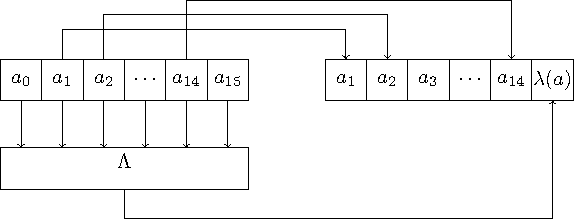
\includegraphics{../pics/kuznyechik/funcLambda.pdf}
    \caption{Hàm $\lambda$}
    \label{kuzfic:1}
\end{figure}

Lưu ý rằng sau khi tính toán trên hàm $\lambda$, đa thức trên
$GF(2^8)$ được chuyển trở lại thành cụm 8 bit sau đó mới
nối vào dãy $a_1$, $a_2$, ..., $a_{15}$ như mô tả ở hình \ref{kuzfic:1}.

Cuối cùng, hàm $L$ ban đầu là thực hiện hàm $\Lambda$ 16 lần.
\[L(a) = \underbrace{\Lambda(\ldots\Lambda(a)\ldots)}_{\text{16 lần}}\]

Như vậy, phép biến đổi trên vòng thứ $i$ với khóa con $k_i$ là
\begin{equation}\label{kuz:4}
    R(k_i, a) = L(S(X(a)))
\end{equation}
với $i = 0, 1, \ldots, 8$.

Ở vòng thứ 10 ta XOR với khóa con $k_9$ nữa: $X(k_9, a)$.

\section{Thuật toán sinh khóa con}

Để sinh khóa con cho 10 lần XOR, thuật toán Kuznyechik dùng mô hình Feistel.
Đầu tiên ta định nghĩa hàm $F(c, a)$. Với $c$ bất kì thuộc $\FF_2^{128}$
và $a = a_0 \Vert a_1$ thuộc $\FF_2^{256}$. Hàm $F(c, a)$ biến phần
tử thuộc $\FF_2^{128} \times \FF_2^{256}$ thành phần tử thuộc 
$\FF_2^{256}$ bằng đẳng thức
\[F(c, a) = a_1 \Vert a_0 \oplus R(c, a_1)\] 
với hàm $R$ được định nghĩa ở phương trình \ref{kuz:4}.

\begin{figure}[ht]
    \centering
    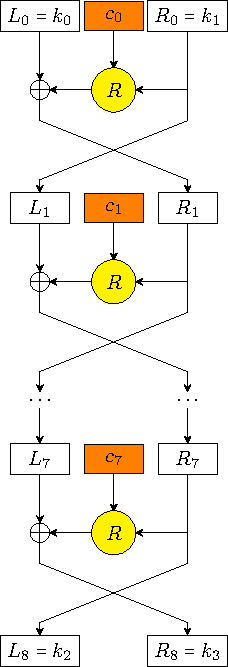
\includegraphics{../pics/kuznyechik/funcF.pdf}
    \caption{Biến đổi từ khóa $k_0 \Vert k_1$ thành $k_2 \Vert k_3$}
    \label{kuzfic:2}
\end{figure}

Với khóa đầu vào là $k \in \FF_2^{256}$, mình ký hiệu ở dạng
ghép 2 chuỗi 128 bit $k = k_0 \Vert k_1$ với $k_0, k_1 \in \FF_2^{128}$ là
những khóa con mở đầu. Khi đó các khóa con cho 10 phép XOR là $k_0$, 
$k_1$, ..., $k_9$.

Thuật toán sinh khóa con được sử dụng như sau
\begin{equation}
    k_{2i+2} \Vert k_{2i+3} = F(c_{8i+7}, \ldots, F(c_{8i}, k_{2i} \Vert k_{2i+1}))
\end{equation}
với $i=0,1,2,3$. Thuật toán có thể mô tả ở hình \ref{kuzfic:2}. Theo đó,
các số $c_0, c_1, \ldots, c_7$ được sử dụng để sinh khóa $k_2 \Vert k_3$
từ $k_0 \Vert k_1$. Tương tự, $c_8, c_9, \ldots, c_{15}$ dược dùng
để sinh khóa $k_4 \Vert k_5$ từ khóa $k_2 \Vert k_3$. Các số $c_0$, $c_1$,
..., $c_{31}$ được định nghĩa trong tiêu chuẩn.

\section{So sánh Kuznyechik với AES}

Điểm giống nhau là cả hai thuật toán đều có phần tuyến tính và 
phần không tuyến tính. Về phần tuyến tính, đối với AES là các
động tác Shift Rows, Mix Columns và Add Round Key, còn đối với
Kuznyechik là hàm $X$ và $L$ bên trên. Về phần không tuyến tính
đều là việc sử dụng một bảng tra cứu SBox của riêng thuật toán đó.

Điểm khác nhau đầu tiên là cách xây dựng ma trận tính toán. Nếu ta
xem xét Shift Rows và Mix Columns dưới dạng phép nhân ma trận 
trên $GF(2^8)$ thì ta thấy rằng ma trận chứa nhiều số 0 nhất có
thể. Điều này giúp tăng tốc độ tính toán. Về phần Kuznyechik, 
phép tính ở hàm $\lambda$ cũng thực hiện trên $GF(2^8)$ nhưng không
chứa bất kì số 0 nào. Điều này làm tăng độ phức tạp tính toán 
nhưng cũng làm tăng tính an toàn.

Điểm khác nhau tiếp theo là việc sinh khóa con. AES sử dụng thuật toán
sinh khóa con từng vòng từ toàn bộ 256 bit ban đầu. Trong khi Kuznyechik
sử dụng mô hình Feistel, theo đó với 256 bit ban đầu được sử dụng cho
2 vòng đầu, cứ mỗi hai khóa con sẽ sinh ra hai khóa con tiếp theo. Như
vậy thuật toán sinh khóa con ít phức tạp hơn AES (Kuznyechik cần 5 lần
sinh khóa còn AES 14 lần).

Vào thời điểm ngày 3 tháng 5 năm 2023 mình chưa đủ trình để đọc các tài
liệu nâng cao về hai hệ mật mã này nên không thể đưa ra đánh giá hay so
sánh về độ an toàn giữa hai hệ mật mã. Tuy nhiên đây là hai tiêu chuẩn 
mã hóa đã qua rất nhiều vòng kiểm định, vậy nên theo góc nhìn của mình
thì rất đáng để nghiên cứu. :D